\documentclass[UTF8, a4paper]{ctexart}
\usepackage[margin=1in]{geometry} % 页边距调整
\usepackage{ctex}
\usepackage{array, amsmath, amssymb}

\usepackage{booktabs, tabularx, multirow, multicol} % 表格拓展支持
\usepackage{graphicx, subfigure, float} % 图片排版支持

\usepackage{algorithm, algpseudocode} % 伪代码支持
\renewcommand{\algorithmicrequire}{\textbf{Input:}}  
\renewcommand{\algorithmicensure}{\textbf{Output:}} 

\usepackage{tikz, mathpazo} % 基本绘图支持
\usepackage{flowchart} % 流程图支持
\usepackage{pgf-umlcd} % UML类图支持
\usetikzlibrary{arrows, shapes, chains, shapes.geometric}

\usepackage{listings} % 代码块支持
\usepackage{xcolor}
\lstset{
	language		= c++,
	backgroundcolor	= \color{white},
	basicstyle		= \footnotesize\ttfamily,
	keywordstyle	= \color{blue},
	stringstyle		= \color{red!58!blue!82}\ttfamily,
	commentstyle	= \color{darkgray},
	rulesepcolor	= \color{red!20!green!20!blue!20},
	columns			= fullflexible,
	breaklines		= true,
	captionpos		= b,
	tabsize			= 4,
	frame			= single,
	escapeinside	= {\%*}{*)}
}
%%示例
% \begin{lstlisting}[caption={}]
% #include <iostream>
% int main(int argc, char *argv[]) {
% 	std::cout << "Hello World!" << std::endl;
% 	return 0;
% }
% \end{lstlisting}

\usepackage{datetime} %日期
\renewcommand{\today}{\number\year{年}\number\month{月}\number\day{日}}

\begin{document}

\begin{center}
	\zihao{3}《数据结构》实验报告
\end{center}
\zihao{5}

\newcolumntype{Y}{>{\raggedleft\arraybackslash}X}
\noindent\begin{tabularx}{\textwidth}{XcY}
	  {班 级:}\;\underline{DL062123}
	& {姓 名:}\;\underline{项乔栋}
	& {学 号:}\;\underline{2021302468} \\
	  {邮 箱:}\;\underline{13282135976@sina.cn}
	& {日 期:}\;\underline{\today}
	& {编 号:}\;\underline{DS09}
\end{tabularx}
~\\

\noindent\textbf{$\circledcirc$
实验题目:\quad{单源最短路径}} \par
\noindent\textbf{$\circledcirc$
实验目的:\quad{解决图论问题}} \par
\noindent\textbf{$\circledcirc$
实验内容:\quad{Dijkstra算法实现单源最短路径的求解}} \par

\subsection*{一、需求分析}
\noindent\fbox{
\begin{tabularx}{\textwidth}{lY}
\bf{Description}
& \parbox[t]{\linewidth}{
	用迪杰斯特拉算法求一点到其余所有结点的最短路径。
} \\

\bf{Input}
& \parbox[t]{\linewidth}{
	先输入一个小于100的正整数n,然后输入图的邻接矩阵(10000表示无穷大,即两点之间没有边),最后输入两个0到n-1的整数表示两个点。
} \\

\bf{Output}
& \parbox[t]{\linewidth}{
	先用迪杰斯特拉算法求给定的第一个点到其余所有结点的最短路径。
	然后再输出给定的两个点之间的最短路径(按顺序输出最短路径上的每一个点,每个数据占一行)。
} \\

\bf{Sample Input}
& \fbox{\parbox[t]{\linewidth}{\bf{
	\mbox{4} \\
	\mbox{0 2 10 10000} \\
	\mbox{2 0 7 3} \\
	\mbox{10 7 0 6} \\
	\mbox{10000 3 6 0} \\
	\mbox{0 2}
}}} \\

\bf{Sample Output}
& \fbox{\parbox[t]{\linewidth}{\bf{
	\mbox{0} \\
	\mbox{1} \\
	\mbox{2}
}}}
\end{tabularx}}

\subsection*{二、概要设计}
% 摘要
\par
1.\;基本操作: \par
	CreateFromIO() $\rightarrow$ Graph \par
	\qquad\textbf{操作结果:}\;从IO流创建无向图 \par
	Dijkstra(G:Graph) $\rightarrow$ Array<Integer> \par
	\qquad\textbf{操作结果:}\;Dijkstra求解单源最短路径 \par
2.\;程序模块: \par
1) 主程序 \par
2) IO支持 \par
3) Dijkstra SSSP问题求解 \par
\begin{figure}[H]
	\begin{minipage}[t]{\linewidth}
		\centering
		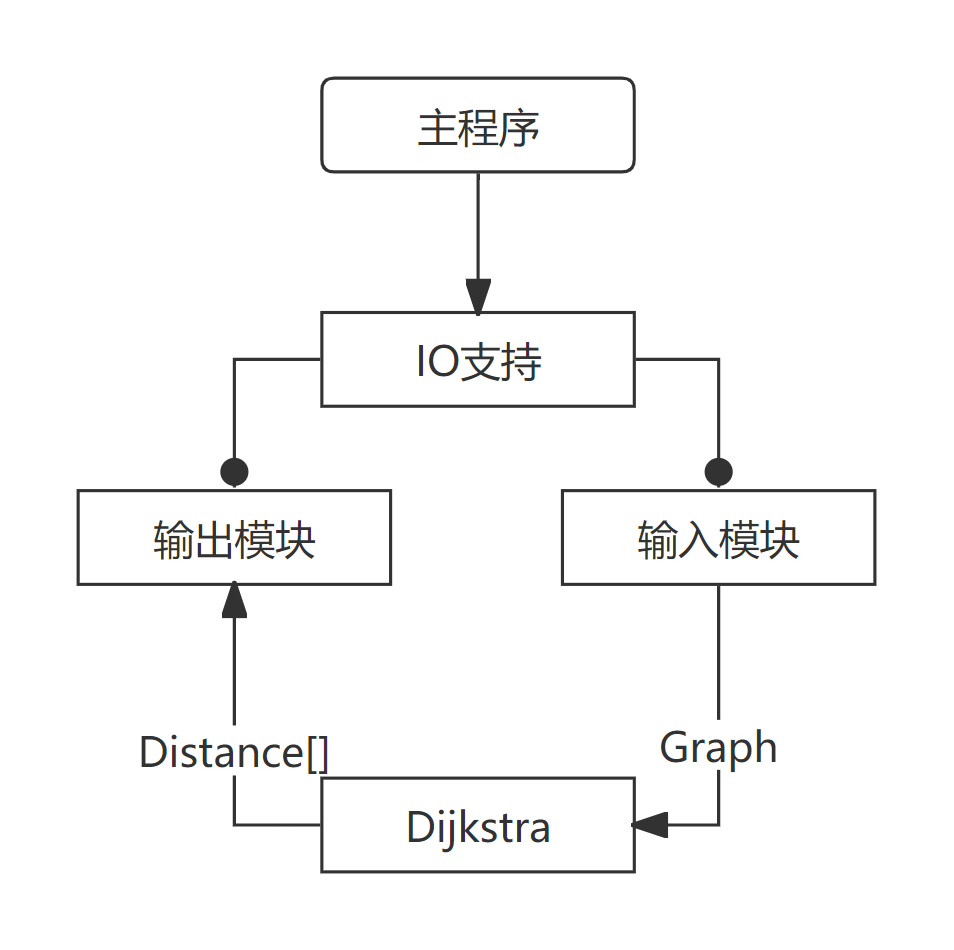
\includegraphics[width=80mm,height=85mm]{./assets/DS09-1}
	\end{minipage}
\end{figure}

\subsection*{三、详细设计}
\begin{algorithm}[H]
\begin{algorithmic}[1]
\caption{SSSP Solution Based on Dijkstra}
\Require UG: $\mathbf{G}$, Source Vertex: $\mathbf{S}$
\Ensure Array<Integer>: $\mathbf{previous}$
\State let $\mathbf{distance}[\mathbf{S}]$ $\gets$ 0
\For {all v $\in$ V($\mathbf{G}$)-\{$\mathbf{S}$\}}
	\State let $\mathbf{distance}[v]$ $\gets$ $\infty$
\EndFor
\For {all v $\in$ V($\mathbf{G}$)}
	\State let $\mathbf{previous}[v]$ $\gets$ nil
\EndFor
\State let Set $\gets$ $\emptyset$
\State let Q $\gets$ V($\mathbf{G}$)
\While {Q $\neq$ $\emptyset$}
	\State let e $\gets$ vertex of minimum distance from Q
	\State let Set $\gets$ Set$\cup$\{e\}
	\For {all v $\in$ neighbors of e}
		\If {$\mathbf{distance}[v]$ > $\mathbf{distance}[e]$ + $\mathbf{G}$[e][v]}
			\State let $\mathbf{distance}[v]$ $\gets$ $\mathbf{distance}[e]$ + $
			\mathbf{G}$[e][v]
			\State let $\mathbf{previous}[v]$ $\gets$ e
		\EndIf
	\EndFor
\EndWhile
\State return $\mathbf{previous}$
\end{algorithmic}
\end{algorithm}

\subsection*{四、使用说明、测试分析与结果}
\subsubsection*{1、使用说明}
1) 本程序可以通过任意支持C++11及以上标准的编译器生成目标文件并在当前平台运行。 \par
2) 进入程序后务必依照需求的输入样式输入数据,手动输入与流式输入都是被允许的。 \par
\subsubsection*{2、测试结果与分析}
2.1\;\textbf{实际环境} \par
对于所有输入,皆为正赋权无向图,且满足输入要求中提及的条件。 \par
2.2\;\textbf{边界情况} \par
无 \par
2.3\;\textbf{测试结果} \par
目标代码通过全部测试,无需纠正 \par
\subsubsection*{3、调试过程问题分析与解决办法}
编码与测试环节皆未产生必须被处理的问题,跳过调试环节 \par
\subsubsection*{4、设计与实现的回顾讨论与分析}
对于初始的Dijkstra的仅仅计算最短路径长度,但是算法过程本身蕴含了最短路径,故要求最短路径,只需在选择最短边时同步保存选边这一信息。而较为简便的做法就是额外保存路径上结点的前向边信息。 \par
\subsubsection*{5、运行界面}
\begin{figure}[H]
	\begin{minipage}[t]{\linewidth}
		\centering
		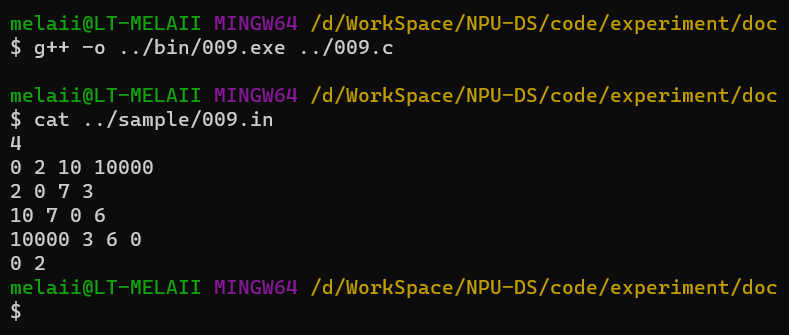
\includegraphics[width=125mm,height=60mm]{./assets/DS09-2}
		\caption{前置环境}
	\end{minipage}
\end{figure}
\begin{figure}[H]
	\begin{minipage}[t]{\linewidth}
		\centering
		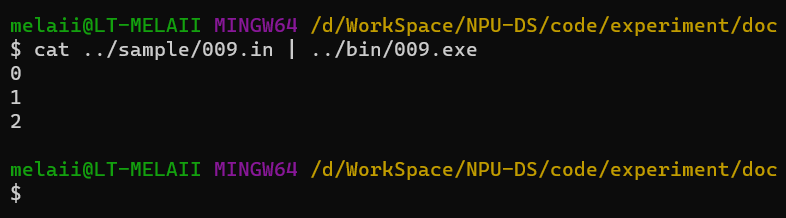
\includegraphics[width=125mm,height=40mm]{./assets/DS09-3}
		\caption{结果输出}
	\end{minipage}
\end{figure}

\subsection*{五、实验总结}
单源最短路径作为一个传统的图论问题,其对应的算法也是极为经典。相较于仅仅求最短路径长度,问题要求求解具体路径,故需要做额外处理的地方仅有在算法执行过程中同步保存边的信息,可以通过一个前向结点的数组来标记一条路径。其余并无太多值得讨论的地方,整体来说算是对Dijkstra算法具体实现代码的一次练手。

~\\
\zihao{-4}
\textbf{教师评语:}
~\\
\textbf{实验成绩:}

\begin{flushright}
\mbox{指导教师签名:\qquad\qquad} \\
\mbox{批阅日期:\qquad\qquad}
\end{flushright}

\end{document}